%%%%%%%%%%%%%%%%%%%%%%%%%%%%%%%%%%%%%%%%%
% Journal Article
% LaTeX Template
% Version 1.4 (15/5/16)
%
% This template has been downloaded from:
% http://www.LaTeXTemplates.com
%
% Original author:
% Frits Wenneker (http://www.howtotex.com) with extensive modifications by
% Vel (vel@LaTeXTemplates.com)
%
% License:
% CC BY-NC-SA 3.0 (http://creativecommons.org/licenses/by-nc-sa/3.0/)
%
%%%%%%%%%%%%%%%%%%%%%%%%%%%%%%%%%%%%%%%%%

%----------------------------------------------------------------------------------------
%	PACKAGES AND OTHER DOCUMENT CONFIGURATIONS
%----------------------------------------------------------------------------------------
%for images

% /\/\/\/\/\/\/\/\/\/\/\/\/\/\/\/\/\/\/\/\/\/\/\/\/\/\/\/\/\/\/\/\/\/\/\/\/\/\/\
%
% THIS IS IMPORTANT! RUN WITH pdflatex -shell-escape TO AVOID EPS CONVERSION ERROR
%
% /\/\/\/\/\/\/\/\/\/\/\/\/\/\/\/\/\/\/\/\/\/\/\/\/\/\/\/\/\/\/\/\/\/\/\/\/\/\/\

\documentclass[twoside,twocolumn]{article}

\usepackage{graphicx}

\graphicspath{ {../img/} } 

\usepackage{subfig}







\usepackage{blindtext} % Package to generate dummy text throughout this template 

\usepackage[sc]{mathpazo} % Use the Palatino font
\usepackage[T1]{fontenc} % Use 8-bit encoding that has 256 glyphs
\linespread{1.05} % Line spacing - Palatino needs more space between lines
\usepackage{microtype} % Slightly tweak font spacing for aesthetics

\usepackage[english]{babel} % Language hyphenation and typographical rules

\usepackage[hmarginratio=1:1,top=32mm,columnsep=20pt]{geometry} % Document margins
\usepackage[labelfont={bf,up},textfont={it,up}]{caption} % Custom captions under/above floats in tables or figures
\usepackage{booktabs} % Horizontal rules in tables

\usepackage{lettrine} % The lettrine is the first enlarged letter at the beginning of the text

\usepackage{enumitem} % Customized lists
\setlist[itemize]{noitemsep} % Make itemize lists more compact

\usepackage{abstract} % Allows abstract customization
\renewcommand{\abstractnamefont}{\normalfont\bfseries} % Set the "Abstract" text to bold
\renewcommand{\abstracttextfont}{\normalfont\small\itshape} % Set the abstract itself to small italic text

\usepackage{titlesec} % Allows customization of titles
\renewcommand\thesection{\Roman{section}} % Roman numerals for the sections
\renewcommand\thesubsection{\roman{subsection}} % roman numerals for subsections
\titleformat{\section}[block]{\large\scshape\centering}{\thesection.}{1em}{} % Change the look of the section titles
\titleformat{\subsection}[block]{\large}{\thesubsection.}{1em}{} % Change the look of the section titles

\usepackage{fancyhdr} % Headers and footers
\pagestyle{fancy} % All pages have headers and footers
\fancyhead{} % Blank out the default header
\fancyfoot{} % Blank out the default footer
\fancyhead[C]{Running title $\bullet$ May 2016 $\bullet$ Vol. XXI, No. 1} % Custom header text
\fancyfoot[RO,LE]{\thepage} % Custom footer text

\usepackage{titling} % Customizing the title section

\usepackage{hyperref} % For hyperlinks in the PDF

\usepackage{amssymb,amsmath,bbold,braket}

%----------------------------------------------------------------------------------------
%	TITLE SECTION
%----------------------------------------------------------------------------------------

\setlength{\droptitle}{-4\baselineskip} % Move the title up

\pretitle{\begin{center}\Huge\bfseries} % Article title formatting
\posttitle{\end{center}} % Article title closing formatting
\title{Simulating a flock of birds} %Simulating a flock of birds
\author{%
\textsc{Steffen Randrup, Michel Smola, Andrei Timus}\thanks{A thank you or further information} \\[1ex] % Your name
\normalsize University of Copenhagen \\ % Your institution
%\normalsize \href{mailto:john@smith.com}{john@smith.com} % Your email address
%\and % Uncomment if 2 authors are required, duplicate these 4 lines if more
%\textsc{Jane Smith}\thanks{Corresponding author} \\[1ex] % Second author's name
%\normalsize University of Utah \\ % Second author's institution
%\normalsize \href{mailto:jane@smith.com}{jane@smith.com} % Second author's email address
}
\date{\today} % Leave empty to omit a date
\renewcommand{\maketitlehookd}{%
\begin{abstract}
\noindent %\blindtext % Dummy abstract text - replace \blindtext with your abstract text


In this paper we present a model for studying the behaviour of a group of particles which have some level of interaction between them. The model was inspired from the $[1]$ paper and as in$ [1]$ the particles have a constant absolute velocity and at each time step  assume the average direction of nearby neighbours with some added perturbation, $\eta$. The behaviour was studied by analysing how the average velocity of the flock $v_a$ varied when parameters like noise, density, number of particles where changed. In addition to $[1]$ we have introduced a cone of vision for every particle and studied the behaviour of the flock in the same conditions. From the simulation results it has been observed that the flock goes through a phase transition where all the particles assume the same direction. The average velocity $v_a$ played the role of an order parameter and it scaled with $(\eta_c-\eta)^\beta$, where $\beta$ is a critical exponent.


\end{abstract}
}

%----------------------------------------------------------------------------------------

\begin{document}



% Print the title
\maketitle

%----------------------------------------------------------------------------------------
%	ARTICLE CONTENTS
%----------------------------------------------------------------------------------------

\section{Introduction}

%\lettrine[nindent=0em,lines=3]{L} orem ipsum dolor sit amet, consectetur adipiscing elit.
%\blindtext % Dummy text

%\blindtext % Dummy text

%------------------------------------------------

The particles where distributed randomly in a square lattice of size L. Each particle had assigned a random direction $\theta$ and a constant interaction radius r. One update consisted in modifying the position of all particles according to the following equation:

\begin{equation}
x_{i}(t+1)=x_i(t)+v_i(t)\Delta t
\end{equation}
where $\Delta$t represents the time between 2 updates.
The velocity of a particle had a constant absolute value and a direction given by:
\begin{equation}
\theta(t+1)=\braket{\theta(t)}_r+\Delta \theta
\end{equation} 

where 
\begin{equation}
\braket{\theta(t)}_r=artan\frac{\braket{sin(\theta(t))}_r}{\braket{cos(\theta(t))}_r}
\end{equation}
is the average direction of the velocities of nearby particles wich are inside the influence circle of radius r of the given particle.$\Delta$t represents the noise in the system and takes values with equal probability within the interval $[-\eta/2,\eta/2]$. For a constant number of particles there are 3 parameters which can be varied: $\eta$,$\rho$,and v, where v is the distance a particle travels between 2 updates.
\begin{figure}[!htb]
	\centering
	\subfloat{{\includegraphics[width=2cm]{test1}}}
	\subfloat{{\includegraphics[width=2cm]{test2}}}
	\qquad
	\subfloat{{\includegraphics[width=2cm]{test2}}}
	\subfloat{{\includegraphics[width=2cm]{test2}}}
	\caption{test for figures}
\end{figure}

Figure 1 shows the configuration of birds for different values of rho and eta. ..........................
..................................


If the density is high enough, while the noise has low values, the system goes through a kinetic phase transition where all the particles share the same direction. In order to study this behaviour we have determined the average normalized velocity of the system and investigated how it changes when certain parameters are modified:
\begin{equation}
v_a=\frac{1}{Nv}\mid\sum_{i=1}^{N} v_i\mid
\end{equation}
For the disordered phase $v_a$ is aproximatively 0, while for the ordered phase $v_a$ has the value of 1.
%rephrase:
In the following figure we show how $v_a$ varies with the noise $\eta$ and density  $\rho$ for a constant value of density and noise respectively.As it can be seen from the graph the overall alignment of the particles depends on the noise and for a high number of particles N the system becomes more disordered. 
%
\begin{figure}[!htb]
	\centering
	\subfloat{{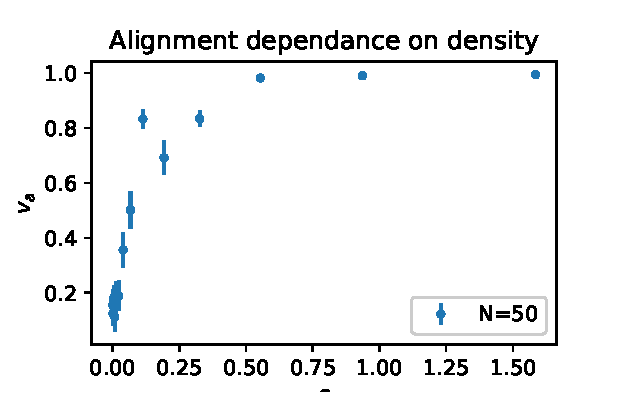
\includegraphics[width=6cm]{va_over_rho}}}
	
	\subfloat{{\includegraphics[width=6cm]{density}}}
	\caption{test for figures}
\end{figure}

The behaviour of $v_a$ is found to be similar to that of the order parameter of some equilibrium systems close to their critical point. For large system sizes the data shows scaling which is an indication of a phase transition. Therefore it's possible to describe the behaviour of $v_a$ in the thermodynamic limit using the following equations:
\begin{equation}
v_a \approx[\eta_c(\rho)-\eta]^\beta 
\end{equation}
\begin{equation}
v_a \approx[\rho-\rho_c(eta)]^\gamma
\end{equation}

\begin{figure}[!htb]
	\centering
	\subfloat{{\includegraphics[width=6cm]{criticaleta}}}

	\caption{test for figures}
\end{figure}


















\section{Results}

Maecenas sed ultricies felis. Sed imperdiet dictum arcu a egestas. 
\begin{itemize}
\item Donec dolor arcu, rutrum id molestie in, viverra sed diam
\item Curabitur feugiat
\item turpis sed auctor facilisis
\item arcu eros accumsan lorem, at posuere mi diam sit amet tortor
\item Fusce fermentum, mi sit amet euismod rutrum
\item sem lorem molestie diam, iaculis aliquet sapien tortor non nisi
\item Pellentesque bibendum pretium aliquet
\end{itemize}
\blindtext % Dummy text

Text requiring further explanation\footnote{Example footnote}.

%------------------------------------------------

\section{Results}

\begin{table}
\caption{Example table}
\centering
\begin{tabular}{llr}
\toprule
\multicolumn{2}{c}{Name} \\
\cmidrule(r){1-2}
First name & Last Name & Grade \\
\midrule
John & Doe & $7.5$ \\
Richard & Miles & $2$ \\
\bottomrule
\end{tabular}
\end{table}

\blindtext % Dummy text

\begin{equation}
\label{eq:emc}
e = mc^2
\end{equation}

\blindtext % Dummy text

%------------------------------------------------

\section{Discussion}

\subsection{Subsection One}

A statement requiring citation \cite{Figueredo:2009dg}.
\blindtext % Dummy text

\subsection{Subsection Two}

\blindtext % Dummy text

%----------------------------------------------------------------------------------------
%	REFERENCE LIST
%----------------------------------------------------------------------------------------

\begin{thebibliography}{99} % Bibliography - this is intentionally simple in this template

\bibitem[Figueredo and Wolf, 2009]{Figueredo:2009dg}
Figueredo, A.~J. and Wolf, P. S.~A. (2009).
\newblock Assortative pairing and life history strategy - a cross-cultural
  study.
\newblock {\em Human Nature}, 20:317--330.
 
\end{thebibliography}

%----------------------------------------------------------------------------------------

\end{document}
